\documentclass[11pt,a4paper,fleqn,twoside]{article}
% Compile doing:
% rm main.aux & rm sections/*.aux & rm main.nlo & rm main.nls & pdflatex main && makeindex main.nlo -s nomencl.ist -o main.nls && bibtex main && pdflatex main && clear && pdflatex main

% Settings
%Personal settings

%Important packages
\usepackage{graphicx}
\usepackage{subfigure}
\usepackage{longtable}
\usepackage{amsmath}
\usepackage{ifthen}

% Additional packages
\usepackage[utf8]{inputenc}
\usepackage[T1]{fontenc}
\usepackage{hyperref}

% Page dimensions
\usepackage[a4paper,inner=2.2cm,outer=2.2cm,bottom=2.2cm,headheight=1cm]{geometry} % to change the page dimensions


%Nomenclature settings
\usepackage{nomencl}
\makenomenclature
\renewcommand{\nomname}{List of symbols}
\newcommand{\nomunit}[1]{\renewcommand{\nomentryend}{\hspace*{\fill}[#1]}}
\newcommand{\mat}[1]{\mathrm{\textbf{#1}}}
\newcommand{\notcien}[2]{$#1\times10^{#2}$}

\renewcommand{\nomgroup}[1]{%
 \ifthenelse{\equal{#1}{A}}{\item[]}{% For roman letters
 \ifthenelse{\equal{#1}{B}}{\item[]}{% For greek letters
 \ifthenelse{\equal{#1}{C}}{\item \vspace{1em} \textbf{Abbreviations}}{% For abbreviations
 \ifthenelse{\equal{#1}{D}}{\item \vspace{1em} \textbf{Configurations}}{}}}}}

%Define which chapters to include
\includeonly{
	sections/Introduction,
	sections/Model_description
	} %{file1,file2,...} 

%%%%%%%%%%%%%%%%%

% Document info
\title{Model description for the implementation of System Identification methodologies on the rotorcraft SH09}
\author{Alejandro Valverde López}


\begin{document}
\maketitle
\tableofcontents

%0.Nomenclature
% [a] -> For roman letters
% [b] -> For greek letters
% [c] -> For abbreviations
% [d] -> For configurations
% Example: \nomenclature[a]{$X$}{Force along x axis\nomunit{N}}
%           \nomenclature[b]{$\alpha$}{angle of attack of the aircraft \nomunit{deg}}
% 
% 
%Aero
\nomenclature[b]{$\alpha$}{Angle of attack \nomunit{deg}}

%Abbreviations
\nomenclature[c]{$CAS$}{Control Augmentation System}
\nomenclature[c]{$CSAS$}{Control and Stability Augmentation System} %Import nomenclature, no text is written
\printnomenclature[0.75in]

%Sections
\clearpage
\section{Introduction}

Bibliography: \cite{Klein2006}, \cite{Remple2006}, \cite{Morelli2011}, \cite{Morelli2011a}

\clearpage
\section{Model description}

\subsection{F-16 model}

This section aims to present the reduced equations for the dynamics of the F-16 fixed-wing aircraft which simulated in a non-linear manner using SIDPAC software.

\subsubsection{Mathematical models of aircrafts}

The notation for the aircraft is the one shown in Figure \ref{fig:aircraftNotation}.

\begin{figure}[!htpb]
  \centering
  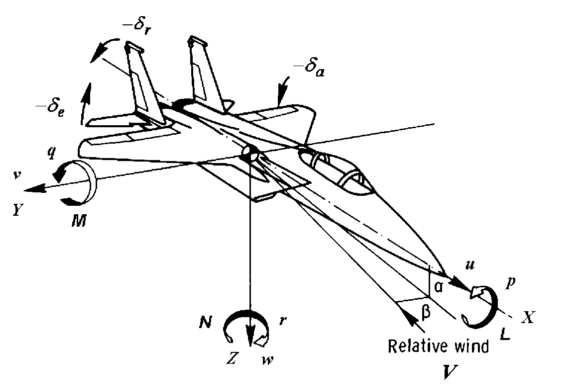
\includegraphics[width=0.7 \textwidth]{figures/aircraftNotation}
  \caption[Airplane notation and sign conventions]{Airplane notation and sign conventions: u, v, w 5 body-axis components of aircraft velocity relative to Earth axes; $p$, $q$, $r$ 5 body-axis components of aircraft angular velocity; $X$, $Y$, $Z$ 5 body-axis components of aerodynamic force acting on the aircraft; and $L$, $M$, $N$ 5 body-axis components of aerodynamic moment acting on the aircraft.}
  \label{fig:aircraftNotation}
\end{figure}

The components of the aerodynamic forces and moments, are the following:

\noindent
Forces:
\begin{eqnarray}
\mathrm{Body \quad axes} \qquad && \mathrm{Stability \quad axes} \\ [6pt]
X = \bar{q}SC_X \qquad && D = \bar{q}SC_D \\ [6pt]
Z = \bar{q}SC_Z \qquad && L = \bar{q}SC_L \\ [6pt]
Y = \bar{q}SC_Y \qquad && Y = \bar{q}SC_Y
\end{eqnarray} 

\noindent
Moments:
\begin{eqnarray}
L = \bar{q} b S C_l \\ [6pt]
M = \bar{q} \bar{c} S C_m \\ [6pt]
N = \bar{q} b S C_n
\end{eqnarray}

\noindent
where $\bar{q}=1/2 \rho V^2$ is the dynamic pressure, $\rho$ is the air density, $V$ is the airspeed, $S$ is the wing reference area, $b$ is the wing span and $\bar{c}$ is the mean aerodynamic chord (MAC). 

The forces expressed in the wind axis systems as shown in set Equations \ref{eq:aeroForcesInWingAxis}. 

\begin{eqnarray} \label{eq:aeroForcesInWingAxis}
\msub{C}{L} = - \msub{C}{Z} \cos \alpha + \msub{C}{X} \sin \alpha \nonumber \\[6pt]
\msub{C}{D} = - \msub{C}{X} \cos \alpha - \msub{C}{Z} \sin \alpha
\end{eqnarray}

The Taylor expansion for the longitudinal motion of the aircraft are expressed in set of Equations \ref{eq:LongitudinalFixedWing}. Hola Eva

\begin{eqnarray} \label{eq:LongitudinalFixedWing}
C_D &=& C_{D_0} + C_{D_V} \frac{\Delta V}{V_0} + C_{D_\alpha} \Delta \alpha + C_{D_q} \frac{q \bar{c}}{2 V_0} + C_{D_{\msub{\delta}{e}} }\Delta \msub{\delta}{e} \nonumber \\ [6pt]
C_L &=& C_{L_0} + C_{L_V} \frac{\Delta V}{V_0} + C_{L_\alpha} \Delta \alpha + C_{L_{\dot{\alpha}}} \frac{\dot{\alpha} \bar{c} }{2 V_0} + C_{L_q} \frac{q \bar{c}}{2 V_0} + C_{L_{\msub{\delta}{e}}} \msub{\delta}{e} \nonumber \\ [6pt]
C_m &=& C_{m_0} + C_{m_V} \frac{\Delta V}{V_0} + C_{m_\alpha} \Delta \alpha + C_{m_{\dot{\alpha}}} \frac{\dot{\alpha} \bar{c} }{2 V_0} + C_{m_q} \frac{q \bar{c}}{2 V_0} + C_{m_{\msub{\delta}{e}}} \msub{\delta}{e} 
\end{eqnarray}

The set of equations that describe the motion of the aircraft, obtained from the Taylor series expansion is the one represented in Equation \ref{eq:LateralFixedWing}.

\begin{eqnarray} \label{eq:LateralFixedWing}
C_Y &=& C_{Y_0} + C_{Y_\beta}\Delta\beta + C_{Y_p}\frac{pb}{2V_0} + C_{Y_r}\frac{rb}{2V_0} + C_{Y_{\msub{\delta}{a}} }\Delta \msub{\delta}{a} + C_{Y_{\msub{\delta}{r}} }\Delta \msub{\delta}{r} \nonumber \\ [6pt]
C_l &=& C_{l_0} + C_{l_\beta}\Delta\beta + C_{l_p}\frac{pb}{2V_0} + C_{l_r}\frac{rb}{2V_0} + C_{l_{\msub{\delta}{a}} }\Delta \msub{\delta}{a} \qquad (C_{l_{\msub{\delta}{r}}} \ll 1) \nonumber \\ [6pt]
C_n &=& C_{n_0} + C_{n_\beta}\Delta\beta + C_{n_p}\frac{pb}{2V_0} + C_{n_r}\frac{rb}{2V_0} + C_{n_{\msub{\delta}{r}} }\Delta \msub{\delta}{r} \qquad (C_{l_{\msub{\delta}{a}}} \ll 1)
\end{eqnarray}


\subsection{Model forces and moments coefficients}
  $\mat{F}$ matrix
  Forces: 
  $$
  X_u, X_v, X_w, X_p, X_q, X_r \\
  Y_u, Y_v, Y_w, Y_p, Y_q, Y_r \\
  Z_u, Z_v, Z_w, Z_p, Z_q, Z_r
  $$

  Moments:
  $$
  L_u, L_v, L_w, L_p, L_q, L_r \\
  M_u, M_v, M_w, M_p, M_q, M_r \\
  N_u, N_v, N_w, N_p, N_q, N_r
  $$

  Controllability, $\mat{G}$ matrix:
  Forces
  $$
  X_{\delta_{\mathrm{lon}}}, X_{\delta_{\mathrm{lat}}}, X_{\delta_{\mathrm{ped}}}, X_{\delta_{\mathrm{col}}} \\
  Y_{\delta_{\mathrm{lon}}}, Y_{\delta_{\mathrm{lat}}}, Y_{\delta_{\mathrm{ped}}}, Y_{\delta_{\mathrm{col}}} \\
  Z_{\delta_{\mathrm{lon}}}, Z_{\delta_{\mathrm{lat}}}, Z_{\delta_{\mathrm{ped}}}, Z_{\delta_{\mathrm{col}}}
  $$

  Moments
  $$
  M_{\delta_{\mathrm{lon}}}, M_{\delta_{\mathrm{lat}}}, M_{\delta_{\mathrm{ped}}}, M_{\delta_{\mathrm{col}}} \\
  N_{\delta_{\mathrm{lon}}}, N_{\delta_{\mathrm{lat}}}, N_{\delta_{\mathrm{ped}}}, N_{\delta_{\mathrm{col}}} \\
  N_{\delta_{\mathrm{lon}}}, N_{\delta_{\mathrm{lat}}}, N_{\delta_{\mathrm{ped}}}, N_{\delta_{\mathrm{col}}}
  $$

  Time delays
  $$
  \tau_{\mathrm{lon}}, \tau_{\mathrm{lat}}, \tau_{\mathrm{ped}}, \tau_{\mathrm{col}}
  $$

% Bibliography
\bibliographystyle{ieeetr}
\bibliography{MyBib}


\end{document}